\documentclass[10pt]{exam}
\usepackage[phy]{template-for-exam}
\usepackage{graphicx}

\title{Sound \#1}
\author{Rohrbach}
\date{\today}

\begin{document}
\maketitle

\begin{questions}

\question
  You have magically been made British and are now at a train station in London getting ready to go out to the country to see your grandparents.  You are walking at a slow pace of 0.5 m/s, and the train (which is stationary) is producing a whistle of 1070 Hz. 


  \begin{parts}
    \part
      If you are on the other end of the station from the train.  As you walk towards it, what frequency will you hear for the whistle?
      \vs 

    \part
      All of a sudden, the train starts to move towards you!  The train continues to make the whistle (at the same 1070 Hz frequency as before), and is traveling at an initial velocity of 7 m/s.  You break out into a dead sprint towards the train at 6.2 m/s.  What frequency will you now hear for the whistle?
      \vs 

    \part 
      You catch up to the train, but it is moving too quickly for you to get on, so it passes you.  You change directions so that you can chase after the train, which is now moving away from you at 22 m/s.  You tap into your inner reserves and are able to get up to a speed of 11.1 m/s.  Now what frequency will you hear for the train?
      \vs 

    \part
      You finally run out of room on the platform and come to an exhausted rest as the train continues out of the station at 41 m/s.  What frequency do you hear for the whistle?
      \vs 

  \end{parts}

\pagebreak
  
\question
  You are on a boat travelling toward a stationary dolphin.  The dolphin whistles at a frequency of 1200~Hz.  You hear a frequency of 1280 Hz.  How fast is your boat travelling?
  \vs[3] 


\question 
  The engine of a racecar emits a relatively constant frequency of 400~Hz.  The racecar has a velocity of 45~m/s.

  \begin{parts}
    \part 
      What frequency do you (a stationary observer) hear as the car approaches?
      \vs[2] 

    \part 
      What frequency do you hear after the car passes?
      \vs[2]

    \part
      Let's say you were Lakitu chasing the car at a speed of 52 m/s.  What frequency would you hear now?

      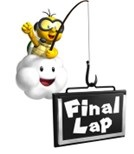
\includegraphics{lakitu.jpg}
      \vs
  \end{parts}



\end{questions}

\end{document}